\documentclass{article}
\usepackage[utf8]{vietnam}
\usepackage{graphicx}
\usepackage{amsmath}
\usepackage{amssymb}
\usepackage{hyperref}
\usepackage{caption}
\usepackage{subcaption}

\title{A realistic fish‑habitat dataset
to evaluate algorithms
for underwater visual analysis \\ \Large Tóm tắt báo tuần 3-4}
\author{Ngọc Thuận - IPSAL LAB}
\date{January 2023}

\begin{document}

\maketitle
\begin{abstract}
    Bài báo này đưa ra một \textit{Dataset} (\textit{DeepFish}) gần với thực tế nhất với nhiều đặc điểm như: kích thước lớn, chất lượng hình ảnh tốt, được thu thập khách quan, phục vụ đa chức năng với mục tiêu phát triển các thuật toán \textit{Computer Vision} và \textit{DeepLearning}\ldots Ứng dụng ra thực tế cho nghiên cứu, nuôi trồng và phát triển ngành thủy sản.
\end{abstract}

    \section{Mục đích chính}
    Có thể tóm tắt mục đích chính của bài báo này như sau:
    \begin{enumerate}
        \item Đưa ra một bộ dữ liệu chuẩn mô tả được độ phức tạp và đa dạng của môi trường tự nhiên dưới nước so với các \textit{datasets} trước đó!
        \item Cung cấp các nhãn bổ sung (\textit{additional labels}) để phân tích toàn diện hơn về các môi trường dưới nước.
        \item Cho thấy tầm quan trọng của việc tiền huấn luyện (\textit{pretrained}) để đạt được các kết quả tốt.
        \item Cung cấp các kết quả để đánh giá các phương pháp mới.
    \end{enumerate}
    \section{Cụ thể}
        Ta sẽ lướt qua những nét nổi bật của bộ dữ liệu này.
        \subsection{Dataset}
        \begin{itemize}
            \item Bắt đầu từ công trình của Bradley và các đồng nghiệp (40 nghìn ảnh).
            \item Mục đích ban đầu không để phục vụ cho các tác vụ Học máy (\textit{Machine Learning}). Nhưng đã được chỉnh sửa thành một cơ sở dữ liệu toàn diện hơn cho lĩnh vực này. Với mong muốn sẽ kích hoạt được các thuật toán mới!
        \end{itemize}
        \subsection{Data collection}
        \begin{figure}[ht!]
            \centering
            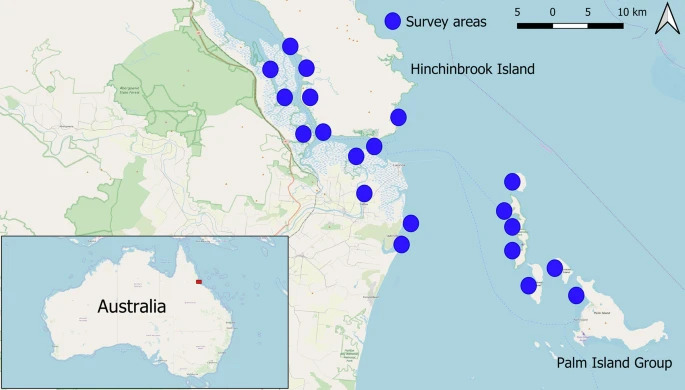
\includegraphics[width = \linewidth]{fig1.jpg}
            \caption{Locations where the DeepFish images were acquired. Most of DeepFish has been acquired from the Hinchinbrook/Palm Islands region in North Eastern Australia, the rest from Western Australia (not shown in the map).
(The map was created using QGIS version 3.8, which is available at https://qgis.org).}
            \label{fig1}
        \end{figure}
        \begin{itemize}
            \item Được thu thập từ 20 môi trường sống khác nhau từ các vùng viên biển xa xôi của vùng nhiệt đới Australia. Hình \ref{fig1}
            \item Quá trình thu thập khách quan khi \textit{camera} được gắn vào mạn tàu sau đó được hạ xuống và giữ khoảng cách $100m$ ghi lại các quần xã tự nhiên dưới nước. Điều này khách quan và hiệu quả hơn trong nghiên cứu và đánh giá so với các phương pháp thu thập dữ liệu khác (ví dụ như lặn, \ldots) 
        \end{itemize}
        \subsection{Additional annotations}
        Ban đầu các nhãn gốc chỉ phù hợp cho các tác vụ phân loại (\textit{classification}) giữa tiền cảnh (\textit{foreground}) và hậu cảnh (\textit{background}), có cá và không có cá (bất kể số lượng). Và việc này không cho phép phân tích loại tiết hơn về môi trường sống. Các chú thích bổ sung ra đời để khắc phục hạn chế này:
        \begin{itemize}
            \item Chú thích cấp điểm (\textit{Point-level annotations}) mục tiêu là giúp mô hình có thể học để đếm cá. Và ứng dụng nó trong việc tự động giám sát quần thể cá (\textit{automatically monitor fish population}), tránh nguy cơ đánh bắt quá mức (\textit{overfishing})
            \item Chú thích cho mỗi \textit{Pixel} (\textit{Per-pixel annotations}) mục tiêu là huấn luyện và đánh giá mô hình để phân đoạn cá trên các hình ảnh. Việc này sẽ hữu ích trong việc ước lượng kích thước, hình dáng, và trọng lượng của cá, và sẽ hữu ích trong việc đánh cá thương mại (\textit{commercial trawling})
        \end{itemize}
        Để ý rằng riêng môi trường \textit{thảm tảo thưa} (\textit{Sparse algal bed}) không có cả hai loại chú thích trên. Lí do là không thể phân biệt rõ ràng giữa cá nhỏ và đá, cũng như một số yếu tố khác.

        \subsection{Dataset splits}
        Chia tập dữ liệu gốc thành các tập con cho các tác vụ của Thị giác máy tính: \textit{FishClf - Classification}, \textit{FishLoc - Counting and Locaization}, \textit{FishSeg - Segmentation}\\
        Mỗi tập dữ liệu con có chia hình ảnh đã được chú thích thành các tập: \textit{training}, \textit{validation} và \textit{test}. Điểm khác là dữ liệu được chia dựa trên môi trường và số lượng quần thể của cá. Trong đó số luôn đảm bảo số ảnh hậu cảnh và tiền cảnh là như nhau, và $50\%$ cho việc huấn luyện, $30\%$ cho việc test và $20\%$ cho việc xác thực.\\
        Kết quả cho ta:
        \\(\textit{training, validation and test})
        \begin{itemize}
            \item 19,3883, 7,953, 11,930 cho \textit{FishClf}
            \item 1,600, 640, 960 cho \textit{FishLoc}
            \item 310, 124, 186 cho \textit{FishSeg}
        \end{itemize}

        \subsection{Comparison to other datasets}
        \begin{figure}[ht!]
            \centering
            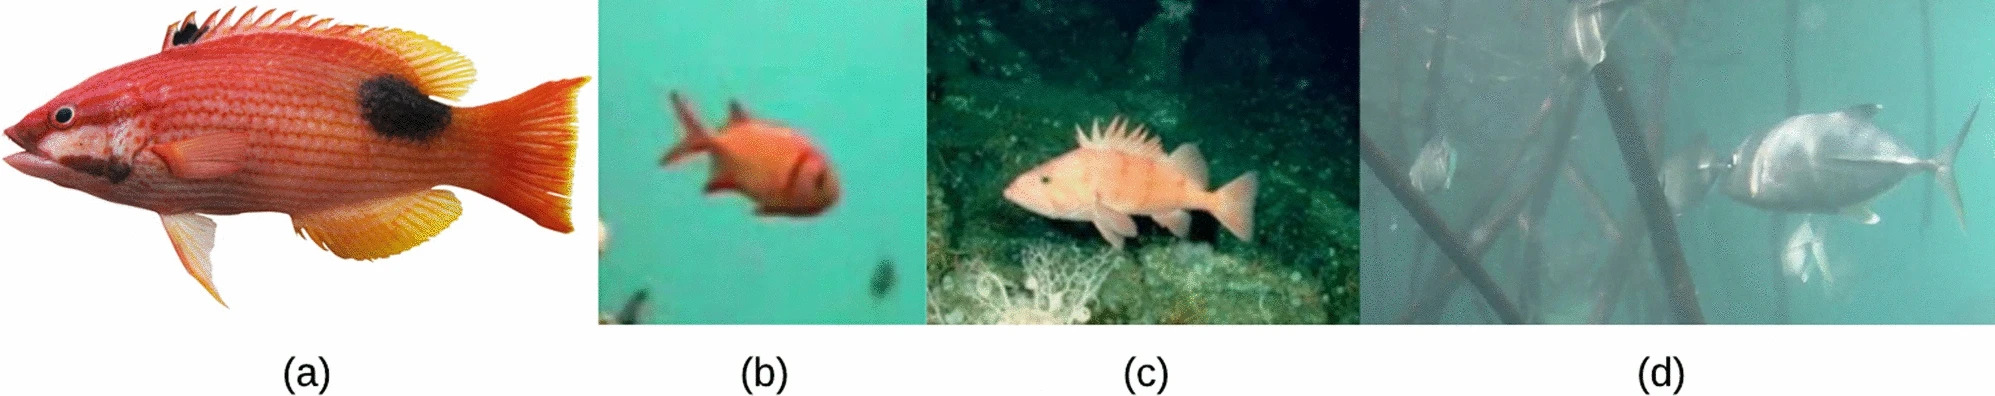
\includegraphics[width = \linewidth]{fig2.jpg}
            \caption{A comparison of fish datasets. (a) QUT1, (b) Fish4Knowledge8, (c) Rockfish35, and (d) our proposed dataset DeepFish. (a–c) Datasets are acquired from constrained environments, whereas DeepFish has more realistic and challenging environments.}
            \label{fig2}
        \end{figure}
        \subsubsection*{Đặc điểm dữ liệu}
            \begin{itemize}
                \item QUT: Đã được hậu chỉnh (\textit{post-processed}) (nền trắng, chỉ cá!)
                \item Rockfish and Fish4Knowledge: Có môi trường đấy, nhưng cá lúc nào cũng ở trọng tâm ảnh
            \end{itemize}
            Còn \textit{DeepFish}:
            \begin{enumerate}
                \item Bao quát về môi trường sống dưới nước của cá
                \item Đa dạng nhiều môi trường sống với các đặc điểm dưới nước khác nhau
                \item Ảnh được thu thập tại chỗ, khách quan, trực tiếp không qua chỉnh sửa
            \end{enumerate}
        \subsubsection*{Tác vụ}
            QUT (\textit{Clf}), Rockfish and Fish4Knowledge (\textit{Detection}). Riêng \textit{DeepFish} một mình 4 tác vụ: Clf, Cnt, Loc, Seg.

        Nhìn chung, bộ dữ liệu \textit{DeepFish} vượt xa các bộ dữ liệu trước đó về kích thước, mức độ phong phú của chú thích cũng như độ phức tạp và biến đổi của ảnh.

        \subsection{Methods and experiments}
        \begin{figure}[ht!]
            \centering
            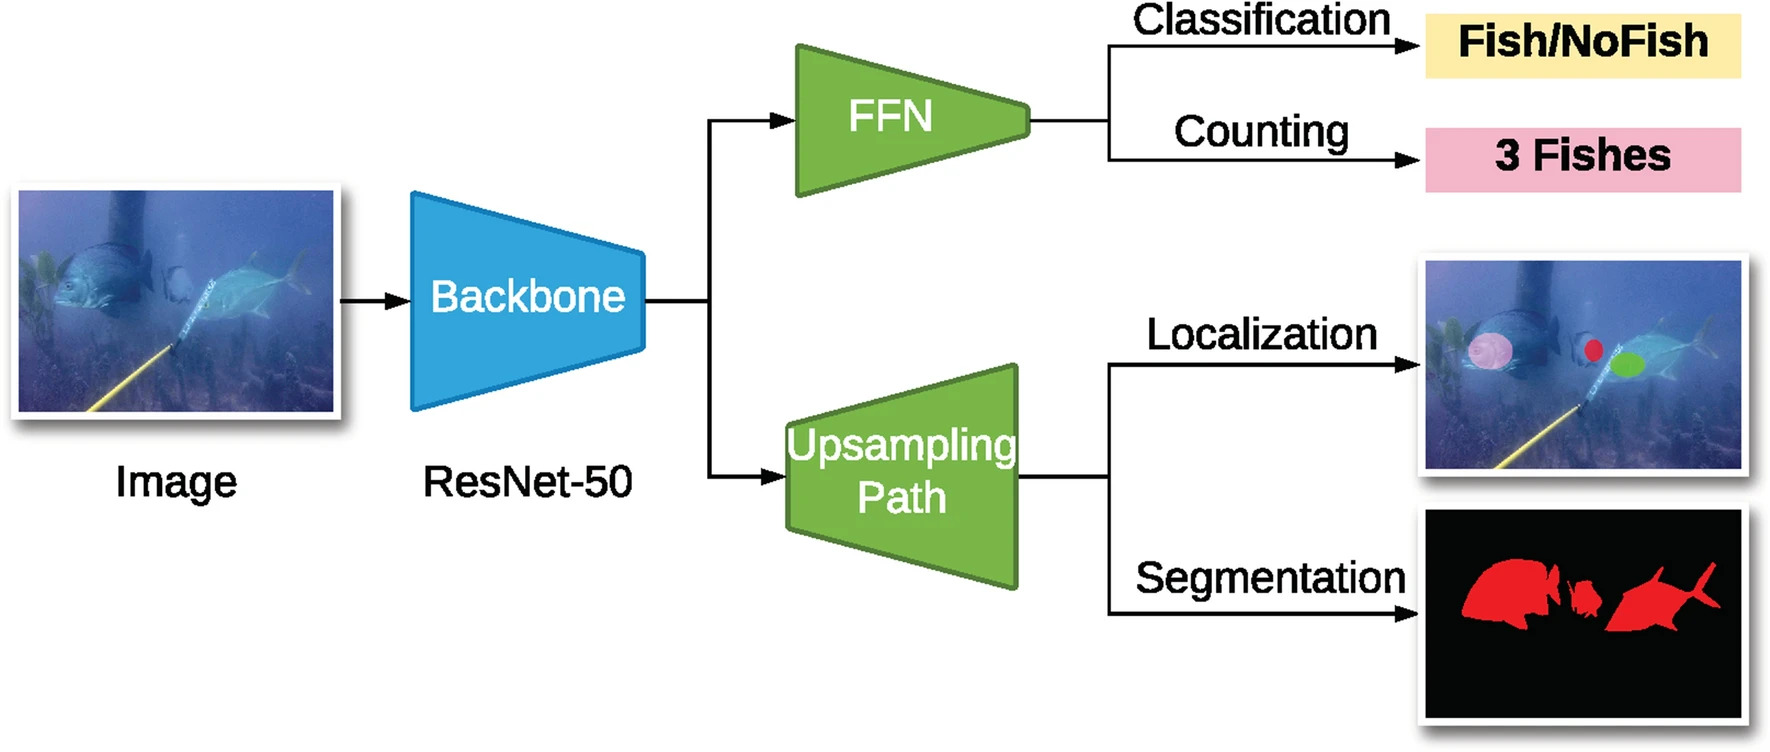
\includegraphics[width = \linewidth]{fig3.jpg}
            \caption{Deep learning methods. The architecture used for the four computer vision tasks of classification, counting, localization, and segmentation consists of two components. The first component is the ResNet-50 backbone which is used to extract features from the input image. The second component is either a feed-forward network that outputs a scalar value for the input image or an upsampling path that outputs a value for each pixel in the image.}
            \label{fig3}
        \end{figure}
        
        Học chuyển tiếp (\textit{Tranfer learning}). Sử dụng \textit{ResNet-50}, \textit{pre-training} bởi \textit{ImageNet}. Khởi tạo ngẫu nhiên \textit{trọng số} (\textit{weights}) cho \textit{ResNet-50} theo phương pháp của Xavier (\textit{Xavier's method}).

        \subsection{Classification results}
        Phân loại: \textit{Foreground} (tiền cảnh - có cá) và \textit{Background} (hậu ảnh - không cá).\\
        Accuracy: $$ACC = \frac{TP+TN}{N}$$
        \\với TP: \textit{True Positives}, TN: \textit{True negatives}, N: the totall number of images. \\Hiểu cơ bản là số lượng phân loại đúng chia tổng số lượng ảnh.
        \begin{enumerate}
            \item Sử dụng \textit{Feed-forward network} (FFN) để tính xác suất.
            \item 3 layers và 2 class output layer
            \item Loss function: \textit{Cross entropy}
            \item Optimizer: \textit{Adam}
        \end{enumerate}
        \ldots

        \subsection{Couting results}
        Sử dụng \textit{mean absolute error} để đánh giá mức độ hiệu quả của mô hình:
        $$ MAE = \frac{1}{N}\sum_{i=1}^{N}|\hat{C_i} - C_i|$$
        trong đó $C_i$ là số lượng cá có trong ảnh, $\hat{C_i}$ là số lượng cá đoán được từ mô hình.\\
        Mô hình đếm khá giống mô hình phân loại, tuy nhiên khác biệt là với mô hình đếm chỉ có một nút đầu ra duy nhất!
        
        \begin{figure}[ht!]
            \centering
            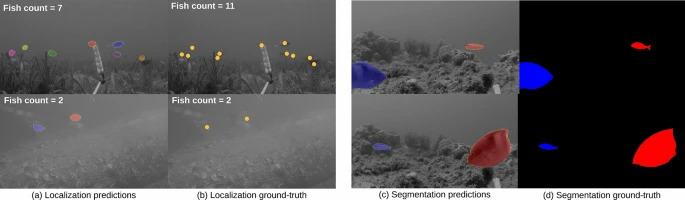
\includegraphics[width = \linewidth]{fig4.jpg}
            \caption{Qualitative results on counting, localization, and segmentation. (a) Prediction results of the model trained with the LCFCN loss21. (b) Annotations that represent the (x, y) coordinates of each fish within the images. (c) Prediction results of the model trained with the focal loss25. (d) Annotations that represent the full segmentation masks of the corresponding fish.}
            \label{fig4}
        \end{figure}
        
        
        \subsection{Localization results}
        Tác vụ này xác định các vị trí có cá trong ảnh, và việc này khó hơn nhiều so với phân loại và đếm bởi đôi khi các con cá còn có thể chồng chéo lên nhau!\\
        Cũng giống với \textit{Couting task} tác vụ này cũng sử dụng dữ liệu trên \textit{FishLoc dataset}, tuy nhiên \textit{MAE} không thể nói lên được độ hiệu quả của mô hình, bởi đôi khi mô hình chọn sai đối tượng nhưng vẫn thỏa mãn. Vì vậy để đánh giá độ chính xác cho tác vụ định vị, ta sử dụng \textit{Grid Average Mean Absolute Error (GAME)}
        $$ GAME = \sum_{i=1}^{4} GAME(L), GAME(L) = \frac{1}{N} \left( \sum_{l=1}^{4^L}|D_{i}^{l} - \hat{D_{i}^{l}}| \right)$$
        trong đó $D_{i}^{l}$ là số lượng chú thích cấp điểm trong vùng \textit{l}, $\hat{D_{i}^{l}}$ là dự đoán của mô hình. \textit{GAME(L)} chia bức ảnh thành một lưới của $4^L$ vùng không chồng lên nhau và sau đó tính tổng điểm \textit{MAE} trên các vùng này.\\
        Tác vụ xác định vị trí chứa \textit{ResNet-50} và \textit{unsampling path}. Và output là xác suất mỗi điểm để rơi vào lớp cá.\\
        Hàm mất mát: \textit{LCFCN}, \textit{LCFCN} được huấn luyện sử dụng 4 chức năng khách quan: \textit{image-level loss, point-level loss, split-level loss} và \textit{false positive loss}. 
        \begin{itemize}
            \item Image-level loss: xác định tất cả những \textit{pixels} là nền của ảnh
            \item Point-level loss: xác định các tâm cá
            \item Split-level loss: dự đoán sao cho một vùng không có quá một chú thích cấp điểm
            \item False possitive loss: ngăn chặt mô hình dự đoán các đốm màu cho các khu vực không có chú thích cấp điểm.
        \end{itemize}

        \subsection{Segmentation results}
        Ta đánh giá mô hình sử dụng chỉ số chuẩn \textit{Jaccard}, là số được định nghĩa là tổng số \textit{pixels} được dự đoán đúng, chia cho tổng số \textit{pixels} được gắn với nhãn với lớp đó. Thường được biết là IoU (\textit{intersection-over-union}), được cho bởi $\frac{TP}{TP+FP+FN}$ \\
        Trong tác vụ này, thay vì sử dụng \textit{cross entropy}, ta sử dụng \textit{focal loss function}, thứ sẽ thích hợp hơn khi mà số lượng pixel hậu cảnh nhiều hơn nhiều cho với pixel tiền cảnh. Còn lại thì sẽ giống với tác vụ xác định vị trí.

        \subsection{Pretrained Model}[ht!]
        \begin{figure}
            \centering
            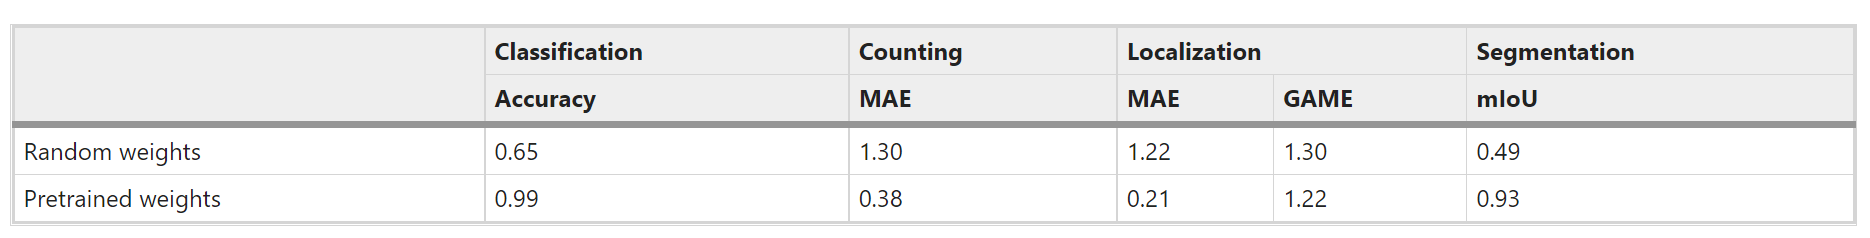
\includegraphics[width = \linewidth]{fig5.png}
            \caption{Classification results were evaluated on the FishClf dataset, counting and localization on the FishLoc dataset, and segmentation on the FishSeg dataset.}
            \label{fig5}
        \end{figure}
        Mô hình tiền huấn luyện thực sự cho kết quả tốt hơn trong tất cả các tác vụ trên.
        \section{Tái bút}
        Đây là lần đầu tôi tóm tắt một bài báo, kiến thức cũng nửa có nửa không so với những kiến thức yêu cầu của bài báo. Cho nên trong quá trình đọc, dịch, hiểu và tóm tắt. Nếu có sai sót nào, xin phép được bỏ qua ạ! Tôi sẽ cố gắng hơn trong các bài sau!
        \section{Bài báo gốc}
        Ta có thể truy cập vào bài báo gốc theo đường link sau:
        \url{https://www.nature.com/articles/s41598-020-71639-x}
\end{document}
